\documentclass[aspectratio=169]{beamer}

\usetheme{Boadilla}
\usefonttheme{professionalfonts}
\setbeamertemplate{navigation symbols}{}
\setbeamertemplate{itemize items}[circle]
\setbeamertemplate{enumerate items}[default]
\setbeamertemplate{headline}{}

\usepackage[utf8]{inputenc}
\usepackage[T1]{fontenc}
\usepackage{lmodern}
\usepackage{amsmath}
\usepackage{booktabs}
\usepackage{tabularx}
\usepackage{array}
\usepackage{hyperref}
\usepackage[strings]{underscore}
\usepackage{listings}
\usepackage{tikz}
\usetikzlibrary{arrows.meta,positioning,fit,calc,shapes.geometric}
\usepackage{xcolor}

\definecolor{courseblue}{HTML}{12355B}
\definecolor{coursegold}{HTML}{C98A2E}
\definecolor{courseice}{HTML}{EEF3F8}
\definecolor{coursegreen}{HTML}{2F6B4F}
\definecolor{coursegray}{HTML}{4B5563}
\definecolor{codebg}{HTML}{F7F9FC}
\definecolor{codecomment}{HTML}{5E6C84}
\definecolor{codestring}{HTML}{0B6E4F}

\setbeamercolor{palette primary}{bg=courseblue,fg=white}
\setbeamercolor{palette secondary}{bg=coursegold,fg=white}
\setbeamercolor{palette tertiary}{bg=courseblue,fg=white}
\setbeamercolor{palette quaternary}{bg=coursegold,fg=white}
\setbeamercolor{structure}{fg=courseblue}
\setbeamercolor{frametitle}{bg=courseice,fg=courseblue}
\setbeamercolor{title}{fg=courseblue}
\setbeamercolor{block title}{bg=courseblue,fg=white}
\setbeamercolor{block body}{bg=courseice,fg=black}
\setbeamercolor{normal text}{fg=black,bg=white}
\setbeamercolor{alerted text}{fg=coursegold}

\setbeamerfont{footline}{size=\scriptsize}

\setbeamertemplate{footline}{
  \leavevmode
  \hbox{
    \begin{beamercolorbox}[wd=.33\paperwidth,ht=2.8ex,dp=1.2ex,leftskip=0.8em]{palette primary}%
      University of Trieste
    \end{beamercolorbox}%
    \begin{beamercolorbox}[wd=.49\paperwidth,ht=2.8ex,dp=1.2ex,center]{palette tertiary}%
      \coursename{} \textbar{} \coursecode
    \end{beamercolorbox}%
    \begin{beamercolorbox}[wd=.18\paperwidth,ht=2.8ex,dp=1.2ex,rightskip=0.8em plus1fil]{palette secondary}%
      \insertframenumber{} / \inserttotalframenumber
    \end{beamercolorbox}%
  }
}

\hypersetup{
  colorlinks=true,
  linkcolor=courseblue,
  urlcolor=coursegreen
}

\lstdefinestyle{coursepython}{
  language=Python,
  basicstyle=\ttfamily\footnotesize,
  keywordstyle=\color{courseblue}\bfseries,
  commentstyle=\color{codecomment}\itshape,
  stringstyle=\color{codestring},
  showstringspaces=false,
  columns=fullflexible,
  keepspaces=true,
  frame=single,
  framerule=0.6pt,
  rulecolor=\color{courseblue},
  backgroundcolor=\color{codebg},
  xleftmargin=0.4em,
  xrightmargin=0.4em,
  aboveskip=0.4em,
  belowskip=0.2em
}

\newcommand{\coursename}{Data-driven Systems Engineering}
\newcommand{\coursecode}{440MI / 305SM}
\newcommand{\coursefooter}{}

\newcommand{\learninggoals}[1]{
  \begin{block}{Learning goals}
  #1
  \end{block}
}

\newcommand{\repoactivity}[1]{
  \begin{block}{Repo activity}
  #1
  \end{block}
}

\newcommand{\readinglist}[1]{
  \begin{block}{Papers and materials}
  {\footnotesize #1}
  \end{block}
}

\newcommand{\coursecontextframe}[5]{
  \begin{frame}{Course Map and Running Cases}
  \centering
  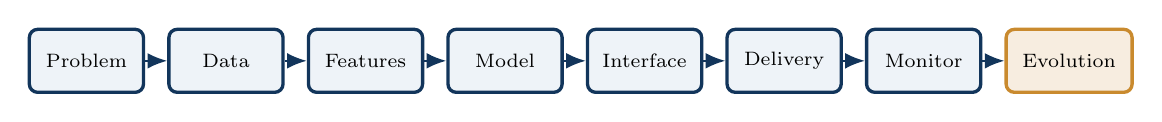
\begin{tikzpicture}[node distance=0.28cm]
  \node[flowbox, minimum width=1.45cm, minimum height=0.8cm] (problem) {\scriptsize Problem};
  \node[flowbox, minimum width=1.45cm, minimum height=0.8cm, right=of problem] (data) {\scriptsize Data};
  \node[flowbox, minimum width=1.45cm, minimum height=0.8cm, right=of data] (features) {\scriptsize Features};
  \node[flowbox, minimum width=1.45cm, minimum height=0.8cm, right=of features] (model) {\scriptsize Model};
  \node[flowbox, minimum width=1.45cm, minimum height=0.8cm, right=of model] (interface) {\scriptsize Interface};
  \node[flowbox, minimum width=1.45cm, minimum height=0.8cm, right=of interface] (delivery) {\scriptsize Delivery};
  \node[flowbox, minimum width=1.45cm, minimum height=0.8cm, right=of delivery] (monitor) {\scriptsize Monitor};
  \node[accentbox, minimum width=1.6cm, minimum height=0.8cm, right=of monitor] (evolution) {\scriptsize Evolution};
  \foreach \a/\b in {problem/data,data/features,features/model,model/interface,interface/delivery,delivery/monitor,monitor/evolution} {
    \draw[arrow] (\a) -- (\b);
  }
  \end{tikzpicture}

  \vspace{0.5em}
  \begin{block}{Today in the course}
  \textbf{Focus:} #1

  \textbf{Bridge:} #2
  \end{block}

  \begin{columns}[T]
  \column{0.48\textwidth}
  \begin{block}{Fraud case}
  {\footnotesize #3}
  \end{block}
  \column{0.48\textwidth}
  \begin{block}{Pasteurization case}
  {\footnotesize #4}
  \end{block}
  \end{columns}

  \vspace{0.3em}
  {\footnotesize \textbf{Course thread:} #5}
  \coursefooter
  \end{frame}
}

\newcommand{\classclosingframe}[4]{
  \begin{frame}{From This Class to the Next}
  \begin{block}{What stays with us}
  #1
  \end{block}

  \begin{columns}[T]
  \column{0.48\textwidth}
  \begin{block}{Project use}
  {\footnotesize #2}
  \end{block}
  \column{0.48\textwidth}
  \begin{block}{Next connection}
  {\footnotesize #3}
  \end{block}
  \end{columns}

  \vspace{0.3em}
  {\footnotesize \textbf{Course thread:} #4}
  \coursefooter
  \end{frame}
}

\tikzset{
  flowbox/.style={
    rounded corners=3pt,
    draw=courseblue,
    fill=courseice,
    very thick,
    minimum width=2.2cm,
    minimum height=0.9cm,
    align=center,
    font=\small
  },
  accentbox/.style={
    rounded corners=3pt,
    draw=coursegold,
    fill=coursegold!15,
    very thick,
    minimum width=2.2cm,
    minimum height=0.9cm,
    align=center,
    font=\small
  },
  arrow/.style={
    -{Latex[length=2.5mm,width=2mm]},
    thick,
    draw=courseblue
  }
}


\title{Class 35: Proposal Presentations, Part 1}
\subtitle{Session 35 of 36 -- Logistics, Rubric, and Course Recap}
\author{\coursename}
\date{18 December}

\begin{document}

\frame{\titlepage \coursefooter}

\begin{frame}{Agenda}
\begin{itemize}
\item Logistics for today's presentations
\item What every presentation must cover
\item Evaluation criteria and rubric
\item Recap: the course arc, Python to Data-Driven to MLOps
\item What we are listening for as reviewers
\end{itemize}
\coursefooter
\end{frame}

\begin{frame}{Today is a defense, not a demo}
\learninggoals{
\begin{itemize}
\item Know the time limit, order, and format for today's presentations.
\item Know exactly what a presentation must cover to be evaluated fairly.
\item Use the rubric to self-check a presentation before presenting.
\item See how today's work is the capstone of the full 36-session arc.
\end{itemize}
}
\coursefooter
\end{frame}

\coursecontextframe
{Presenting and defending a scoped project plan.}
{Today and Class 36 are one event split across the same day: this is where the pitch from Class 32 and the plan from Class 34 meet an audience.}
{Teams presenting a fraud-pattern project should show how their own data and constraints diverge from the class example, not just repeat it.}
{Teams presenting a pasteurization-pattern project should do the same: use the class case as a template, not a fixed answer.}
{The course began with a systems view, problem through evolution; today each team shows that arc applied to a project of its own.}

\begin{frame}{Logistics for today}
\begin{itemize}
\item Each team presents for 10 minutes, followed by 5 minutes of questions.
\item Teams present in the order posted before class; be ready 5 minutes before your slot.
\item Bring slides plus, if available, a short live or recorded demo; a working screenshot is an acceptable fallback.
\item If your team is not presenting today, you are still an active reviewer: written feedback is expected from everyone.
\end{itemize}
\coursefooter
\end{frame}

\begin{frame}{What every presentation must cover}
\begin{itemize}
\item Problem statement and target users, in plain language.
\item Data source and how it was or will be accessed.
\item MVP scope, shown or demoed if at all possible.
\item A glimpse of the milestone sequence and current position in it.
\item The top two risks and how the team plans to handle them.
\item One concrete success criterion for the finished project.
\end{itemize}
\coursefooter
\end{frame}

\begin{frame}{Evaluation criteria}
\begin{tabularx}{\textwidth}{>{\bfseries}l X}
Criterion & What reviewers look for \\
\toprule
Problem clarity & A specific problem and user, not a vague topic area. \\
Feasibility & Scope matches the time and data actually available. \\
Lifecycle coverage & Requirements, delivery, and monitoring are at least sketched, not only modeling. \\
Risk awareness & Real risks are named, with a plausible response. \\
Communication & The team can explain choices and answer questions clearly. \\
\bottomrule
\end{tabularx}
\coursefooter
\end{frame}

\begin{frame}{Recap: the course arc}
\centering
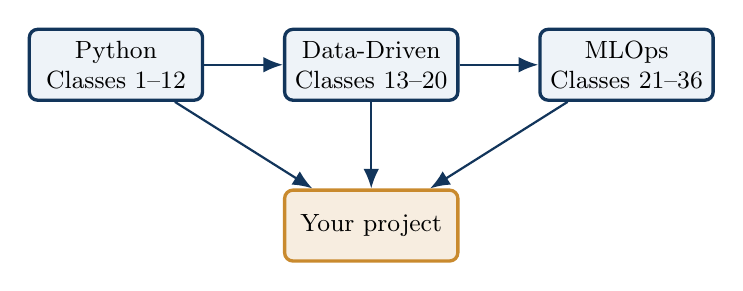
\begin{tikzpicture}[node distance=0.9cm and 1cm]
\node[flowbox] (py) {Python\\Classes 1--12};
\node[flowbox, right=of py] (dd) {Data-Driven\\Classes 13--20};
\node[flowbox, right=of dd] (ml) {MLOps\\Classes 21--36};
\node[accentbox, below=1.1cm of dd] (project) {Your project};
\draw[arrow] (py) -- (dd);
\draw[arrow] (dd) -- (ml);
\draw[arrow] (py) -- (project);
\draw[arrow] (dd) -- (project);
\draw[arrow] (ml) -- (project);
\end{tikzpicture}
\vspace{0.4em}
\begin{itemize}
\item Every block you sat through is supposed to show up somewhere in what you present today.
\end{itemize}
\coursefooter
\end{frame}

\begin{frame}{What we are listening for as reviewers}
\begin{itemize}
\item Clarity: could someone outside this course understand the problem in one sentence?
\item Honesty: does the team acknowledge what is not yet working or not yet known?
\item Defensibility: can choices be justified, even if a reviewer disagrees with them?
\end{itemize}
\coursefooter
\end{frame}

\begin{frame}{What your project repo should show today}
\repoactivity{
\begin{itemize}
\item A README describing the problem, data, and how to run what exists so far.
\item A dependency file, such as `requirements.txt`, matching what the code actually uses.
\item At least one runnable entry point, even if it only runs a baseline or a stub service.
\end{itemize}
This is the same repo hygiene the course has used throughout, now applied to your own project.
}
\coursefooter
\end{frame}

\begin{frame}{Discussion prompt}
\begin{block}{Question}
As an audience member today, write down one question you would want asked of your own project.
\end{block}
\begin{itemize}
\item This turns passive listening into active review.
\item It also prepares you for the questions your own team will get.
\end{itemize}
\coursefooter
\end{frame}

\begin{frame}{Papers and materials}
\readinglist{
The three anchor texts for the whole course, useful again while you scope and defend your own project:\
\href{https://www.pearson.com/en-us/subject-catalog/p/software-engineering/P200000003144/9780137035151}{Sommerville, Software Engineering};\
\href{https://www.oreilly.com/library/view/designing-machine-learning/9781098107956/}{Chip Huyen, Designing Machine Learning Systems};\
\href{https://www.oreilly.com/library/view/practical-mlops/9781098103002/}{Practical MLOps}.
}
\coursefooter
\end{frame}

\classclosingframe
{\begin{itemize}
\item A good presentation shows a bounded problem, a realistic plan, named risks, and honest status.
\item The rubric rewards lifecycle thinking, not only a working model.
\item Reviewing other teams sharpens what you notice about your own project.
\end{itemize}}
{Your feedback today, given and received, should directly update your milestone plan from Class 34.}
{Class 36 continues the same event this afternoon: same rubric, same format, remaining teams.}
{One rubric, applied consistently across both halves of today, closes the loop from Class 32's pitch to a defended plan.}

\end{document}
